\documentclass[10pt]{article}
\usepackage[T1]{fontenc}
\usepackage{amsmath,amssymb,graphicx,booktabs,longtable}
\usepackage[margin=0.9in]{geometry}
\usepackage[hidelinks]{hyperref}
\title{A Counterexample to Scalar Smoothing-Error Representations\\in Lorentz-Cone Contact Models}
\author{Suneet Dungrani\\Independent Researcher\\\texttt{suneetdungrani@utexas.edu}}
\date{FORGE-CONEBOUND\\November 2026}
\hypersetup{pdftitle={A Counterexample to Scalar Smoothing-Error Representations in Lorentz-Cone Contact Models},pdfauthor={Suneet Dungrani},pdfsubject={FORGE-CONEBOUND},pdfkeywords={Lorentz cones, smoothing error, contact models, convex optimization, exact arithmetic}}
\begin{document}
\maketitle
\begin{abstract}
This study examines whether one scalar multiplier per vector contact can represent smoothing error in a fixed strongly convex conic model. An exact three-dimensional Lorentz-cone family requires unequal spectral multipliers, excluding the hard optimizer from the proposed one-generator segment. A six-coordinate substitution satisfies the displayed structured equations of the audited source. The construction is algebraic; no physical robot failure is demonstrated. Two spectral generators repair the isotropic separated case; ordinary primal--dual gap ellipsoids provide a standard general alternative. A standalone implementation checks small exact rational problems, preserves unsuccessful numerical attempts, and separates ideal mathematical failures from rounded implementation-set separations. The frozen evaluation contains 240 held-out base problems, six nested smoothing levels, separate stress controls, and 30 paired timing repeats on 50 preselected bases. Neither alternative met the complete predefined efficiency criterion; no efficiency improvement is claimed.
\end{abstract}
\noindent\textbf{Keywords:} Lorentz cones; smoothing-error bounds; contact models; convex optimization; exact arithmetic.


\section{Introduction}
The target is the scalar-per-contact representation in Li and Chou's equations (6)--(7)\cite{li2026rss,li2026arxiv}. The RSS proceedings version, arXiv versions and pinned public implementation were inspected. The final proceedings statement retains one scalar per contact and the cross-contact independence condition. The arXiv appendix and implementation use the half-log Lorentz barrier. The inspected code builds one disturbance column per contact; the code itself and the reported robotics experiments were not compiled or rerun here. The result concerns the written structured conic equations and an independent mathematical implementation.

The result identifies a limitation of scalar smoothing-error bounds rather than introducing a general contact solver. Generic gap localization is established convex optimization, with dual safe-region constructions appearing in Gap Safe\cite{gap} and RYU\cite{ryu}. Parametric optimizer-set reachability\cite{gould} addresses uncertainty in problem parameters; the problem studied here has fixed coefficients. The two-generator construction follows from elementary spectral calculus. The contribution is the exact scalar-representation counterexample and its algebraic relationship to the audited model; no general new localization theorem or global priority claim is made.

\section{Model and exact counterexample}
Let $L_3=\{r:r_0\geq\sqrt{r_1^2+r_2^2}\}$, and consider
\[
 \min_{r\in L_3}\ \tfrac12\|r\|_2^2+c^\top r,
 \qquad c=(2,1,0).
\]
Since $c$ is strictly in the self-dual cone, the unique hard optimum is $r_*=0$. Use $\psi(r)=-\tfrac12\log(r_0^2-\|r_t\|^2)$. With $e_\pm=(1,\pm1,0)/2$ and
\[
 t_\beta(\kappa)=\frac{\sqrt{\beta^2+4\kappa}-\beta}{2},
 \qquad t'_\beta(\kappa)=\frac1{\sqrt{\beta^2+4\kappa}},
\]
the unique smoothed solution is $r_\kappa=t_3e_++t_1e_-$ and its dual is $r_\kappa+c$. These satisfy stationarity and Jordan complementarity exactly. If $0\in r_\kappa-\kappa r'_\kappa[1,2]$, one common scalar must equal both
\[
 w_\beta=\frac{2\sqrt{\beta^2+4\kappa}}
 {\sqrt{\beta^2+4\kappa}+\beta},\qquad \beta=3,1.
\]
But $\beta/\sqrt{\beta^2+4\kappa}$ is strictly increasing for positive $\beta$, so $w_3<w_1$ for every $\kappa>0$. Equivalently, the squared positive ratios satisfy $9/(9+4\kappa)>1/(1+4\kappa)$, since cross multiplication gives $32\kappa>0$. No common scalar exists, even without limiting it to $[1,2]$. At $\kappa=1$, the recorded 80-digit calculation gives a segment miss of 0.0483821540743481. The decimal calculation corroborates the exact argument and is not interval arithmetic.

\paragraph{Source-coordinate substitution.}
Set the friction coefficient to $\mu=1$. Take $P=2I_6$, $q=(-c,c)$, $J=[-I_3\ I_3]$, $b=0$. With $r=x_o-x_a$ and $m=(x_a+x_o)/2$, the objective becomes $2\|m\|^2+\|r\|^2/2+c^\top r$. Thus $m=0$ and $JP^{-1}J^\top=I_3$. The source's displayed Appendix B coefficients are obtained with $K_a=2I_3$, $M_o/\Delta t^2=2I_3$, $u=c/2$, $\tau_a=0$, $\tau_o=-c$, and initial state/gap zero. In the force convention, $\lambda_\kappa=c+r_\kappa$ and $\lambda_*=c$. Here $f_\kappa=(-r_\kappa/2,r_\kappa/2)$, $f_0=0$, and $P^{-1}J^\top z=(-z/2,z/2)$, so source equation (6) would require $r_\kappa=\kappa r'_\kappa w$. One contact satisfies every intercontact zero condition vacuously. This algebraic substitution does not establish physical realizability or a hardware safety consequence.\footnote{Pinned source: \href{https://github.com/trustworthyrobotics/quasistatic-contact-SLS/tree/e7995fc8293ffd7d97047506b48ad948b9d35984}{\texttt{quasistatic-contact-SLS}, commit \texttt{e7995fc8}}; full identifier in the supplement.}

\paragraph{Cartesian factors are insufficient.}
At $\kappa=2$, the tangential coordinate and derivative are $(\sqrt{17}-5)/4$ and $(1/\sqrt{17}-1/3)/2$. The multiplier needed to recover zero exceeds two: the inequality reduces to $27<7\sqrt{17}$, verified by $729<833$. Independent physical-coordinate factors therefore do not supply a general repair.

\begin{figure}[t]\centering
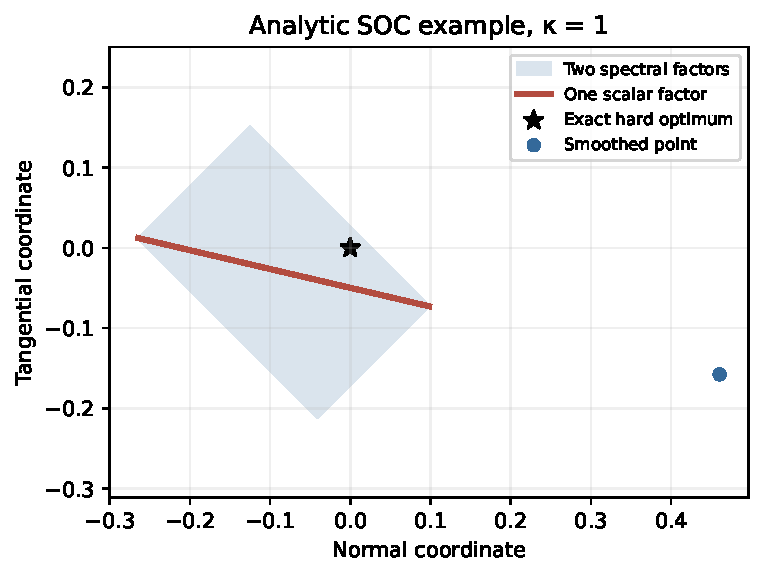
\includegraphics[width=.64\linewidth]{figures/spectral_geometry.pdf}
\caption{Analytic dimensionless illustration. The hard optimum lies outside the scalar segment and inside the restricted spectral set. This is not a robot experiment.}
\end{figure}

\section{Valid alternatives and arithmetic}
For an isotropic metric $\alpha I$ with $\alpha>0$, write $\beta_\pm=c_0\pm\|c_t\|$, $t_j=(R_j-\beta_j)/(2\alpha)$, $t_{0,j}=\max\{-\beta_j/\alpha,0\}$ and $t'_j=1/R_j$. Fixed spectral coordinates give
\[
 t_j-t_{0,j}=\kappa t'_j\frac{2R_j}{R_j+|\beta_j|},
 \quad R_j=\sqrt{\beta_j^2+4\alpha\kappa},
 \quad 1\leq\frac{2R_j}{R_j+|\beta_j|}\leq2.
\]
Independent spectral factors therefore enclose the hard optimum. The spectral construction applies only to separated isotropic blocks, with $J=I$ and $b=0$. It rejects arbitrary whitening, anisotropic or coupled use. Floating-point generator coefficients remain numerical outputs.
At repeated eigenvalues the hard and central points are independent of the chosen spectral frame; the outer zonotope and its directional widths can depend on that frame, while the inclusion remains valid.

For the fixed problem $\min\tfrac12v^\top Pv+q^\top v$ with $P\succ0$ and $Jv+b\in K$, where $K$ is a product of Lorentz and nonnegative cones, let $\hat v$ and $y\in K^*=K$ be feasible primal/dual witnesses, $a=J^\top y-q$, $v_d=P^{-1}a$, and $d(y)=-a^\top v_d/2-b^\top y$. Weak duality\cite[Section 5.1.3]{boyd2004} and completion of the quadratic Lagrangian square give
\[
 (v_*-v_d)^\top P(v_*-v_d)\leq2g,
 \qquad g=f(\hat v)-d(y)\geq0.
\]
Support in direction $h$ is bounded by $h^\top v_d\pm\sqrt{2g h^\top P^{-1}h}$. Exact rational LDL, cone inequalities, linear solves and integer-verified outward square roots establish certificates for the rational problem obtained by exact conversion of the supplied binary64 coefficients. This certifies that binary-input problem, without measurement uncertainty. Boundary feasible witnesses are allowed. Negative computed gaps are rejected; logged witness modifications are rechecked exactly. An independent implementation uses Sylvester determinants and exact support inequalities to replay the certificates.

\section{Frozen bank and protocol-corrected replication}
The first execution used the frozen experimental implementation. A subsequent protocol correction addressed an incomplete high-precision-library warmup, optional-solver availability reporting, an adapter capability flag, a baseline-validation condition and incomplete subprocess resource accounting. A second full execution corrects those protocol/software seams in a fresh environment. Optimizer equations, solver settings, matrices, timing order, selection and metric thresholds are unchanged. The corrected execution was selected before its outcomes for the reported operational measurements, regardless of favorable or unfavorable performance. Both cohorts and their differences are retained; they are paired replications of the same cases, not a doubled independent sample. The corrected execution is a post-outcome protocol repair rather than a strictly preregistered new experiment.
The five synthetic families are: one isotropic Lorentz cone; one anisotropic cone; separated multi-cone blocks; mixed coupled metrics with zero-coupling controls; and affine mixed cones with known strict feasible points. There are 48 held-out base problems per family. The six shared levels are $10^{-6},10^{-4},10^{-2},1,10,100$. Development uses a separate 60-problem bank. The 36 stress fixtures and deterministic controls are excluded from the random-frequency denominator.

B0 is direct hard projection on its domain; B1 is a public hard conic solve plus exact gap validation; B2 is the scalar audit target; B3 is the invalid Cartesian control; M1 is restricted spectral construction; M2 is a standard gap enclosure from the smoothing solve. The smoothing reference retains unsuccessful float attempts and may use 70-digit continuation, sharing its iteration/time budget. Method cost starts from in-memory coefficient payloads and includes parsing, validation, factorization, solving, enclosure construction and checks; process startup and library imports are excluded. Library and high-precision code paths are warmed before cold solver-state repeats, with BLAS threads fixed to one. Warm-start diagnostics are separate.

Base problems are the statistical units. Kappa values, directions and timing repeats are nested. Timing uses the 50 preselected bases and 30 repeats at every kappa. Paired bootstrap resamples retain base identities within the declared design cells, with 10,000 draws and disclosed sparse cells. A failed or undecided case is retained. A rounded set's validated separation is distinct from an ideal source-set proof. Frequency bounds keep unascertained inclusion outcomes unknown.

\section{Results}
The paired cohort check records 0 discrepancies in status, mathematical certificate, diagnostic or numerical vector under the declared comparison tolerance. Every discrepancy, if present, remains in the comparison artifact. The table below gives descriptive full-method costs: medians over 30 repeats at each level, then over the six levels for each base, then over 50 bases. The 95th percentile uses these base summaries. Unsupported and failed attempts remain included in these cost descriptions; this table is not evidence of a matched-quality speed advantage.

\begin{center}\small
\begin{tabular}{lrrrr}\toprule
Method & Original median ms & Corrected median ms & Corrected p95 ms & Paired ratio\\\midrule
B0 & 0.1163 & 0.1219 & 0.2039 & 1.025 \\
B1 & 2.374 & 2.487 & 34.93 & 1.008 \\
B2 & 1.259 & 1.254 & 172.5 & 1.028 \\
B3 & 1.244 & 1.273 & 170.4 & 1.028 \\
M1 & 0.1848 & 0.191 & 0.2771 & 1.02 \\
M2 & 3.805 & 3.857 & 176 & 1.011 \\
\bottomrule\end{tabular}\end{center}

The table reports method attempts, including unsupported domains and numerical failures. The following counts are nested base--kappa observations; they are not independent trials. The base-frequency table uses one unit per base problem and keeps unascertained cases unknown. Exactly 20484 gap outputs were covered by independent replay in the held-out and timing artifacts, comprising 1674 distinct complete input/output payloads. Repeated identical payloads were checked once after exact-payload identity verification.

\begin{center}\small
\begin{tabular}{lrrrrr}\toprule
Method & Validated & Numerical & Unsupported & Failed & Undecided\\\midrule
B0 & 0 & 432 & 1008 & 0 & 0 \\
B1 & 1404 & 0 & 0 & 36 & 0 \\
B2 & 0 & 1440 & 0 & 0 & 0 \\
B3 & 0 & 1440 & 0 & 0 & 0 \\
M1 & 0 & 432 & 1008 & 0 & 0 \\
M2 & 1440 & 0 & 0 & 0 & 0 \\
\bottomrule\end{tabular}\end{center}
Each method has 1,440 held-out base--level attempts. Numerical means numerical-only evidence; undecided denotes the INDETERMINATE status. The complete 30-row family--method table, including rounded-set misses and ideal proofs, is retained in the accompanying \texttt{supplement.pdf}.

\begin{center}\small
\begin{tabular}{lrrrrrr}\toprule
Family & Bases & \shortstack{Source\\eligible} & \shortstack{Rounded\\miss} & \shortstack{Rounded\\unknown} & \shortstack{Ideal source\\miss} & \shortstack{Ideal\\unknown}\\\midrule
F1 & 48 & 48 & 48 & 0 & 19 & 29 \\
F2 & 48 & 48 & 42 & 6 & 0 & 48 \\
F3 & 48 & 48 & 42 & 6 & 0 & 48 \\
F4 & 48 & 12 & 46 & 2 & 0 & 48 \\
F5 & 48 & 0 & 39 & 9 & 0 & 48 \\
\bottomrule\end{tabular}\end{center}
The base-frequency table reports any B2 miss across the six nested levels. Known misses form a lower bound; adding unknown bases gives the upper identification bound. Counts outside the source assumption do not refute that assumption-restricted theorem. These are properties of the declared synthetic generator, rather than estimates of robot failures.

\begin{figure}[t]\centering
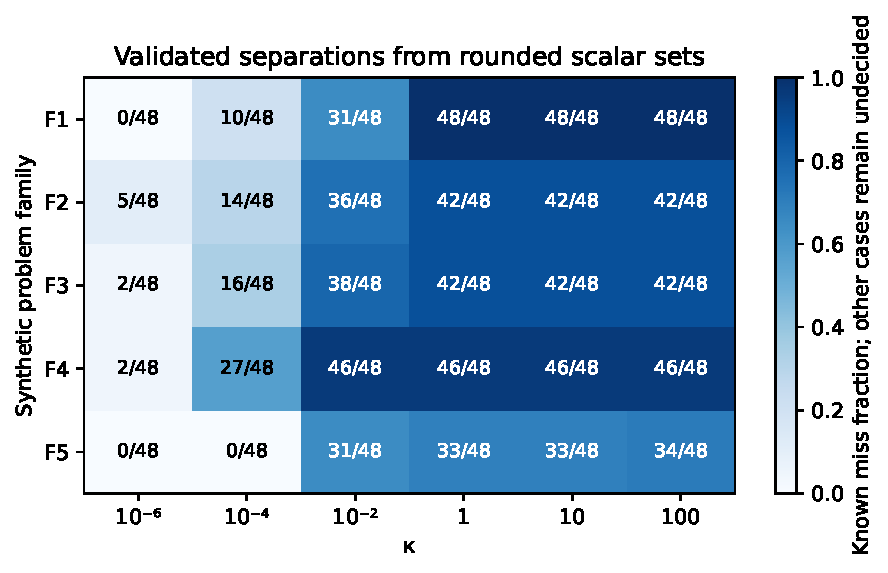
\includegraphics[width=.9\linewidth]{figures/scalar_failure_map.pdf}
\caption{Known separations from rounded scalar implementation sets. Other outcomes remain undecided for rigorous containment. Source eligibility is tracked separately; coupled examples alone do not refute an independent-contact theorem.}
\end{figure}

The efficiency threshold requires at least 25\% median paired savings with a 95\% lower bootstrap bound above 10\%, matched validation/accuracy, no certificate errors, and an equal-family, equal-base mean fraction of at least 95\% of paired directional width ratios no larger than 1.25. Neither alternative met the complete predefined efficiency criterion; no efficiency improvement is claimed. Undefined widths and missing comparisons remain explicit rather than being clipped.

\begin{center}\small
\begin{tabular}{llllp{3cm}}\toprule Method & Median saving & 95\% interval & Width fraction & Gate\\\midrule
M1 & undecided & undecided & undecided & not established \\
M2 & undecided & undecided & undecided & not established \\
\bottomrule\end{tabular}\end{center}

\begin{figure}[t]\centering
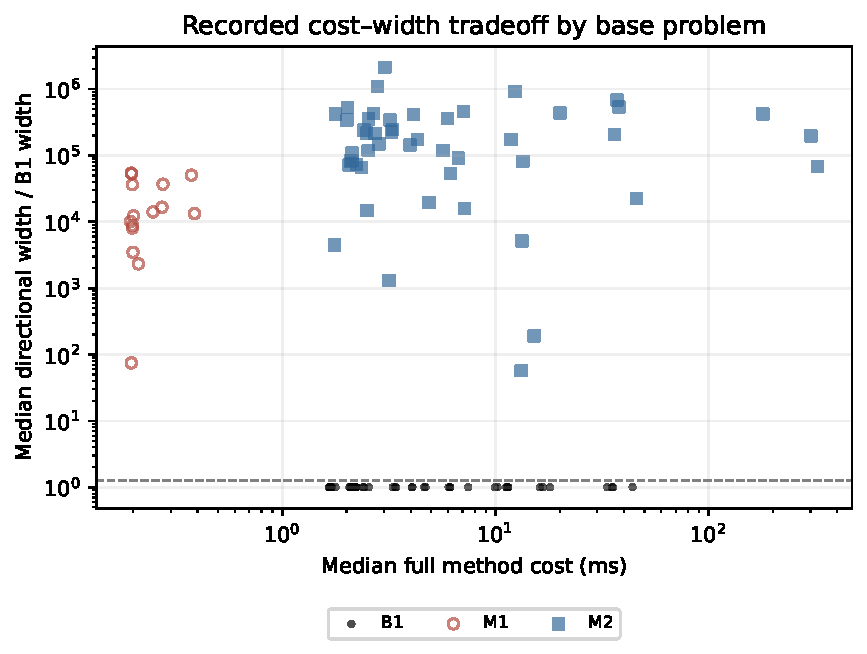
\includegraphics[width=.8\linewidth]{figures/width_runtime.pdf}
\caption{Recorded full cost--width tradeoff by base problem. M1 has numerical coefficients. Undefined/non-operational points and all method statuses are accounted for in the tables and figure manifest.}
\end{figure}

\section{Limitations and interpretation}
The exact counterexample establishes failure of the stated scalar representation on the written fixed-conic model. It does not establish an error rate for real robots, invalidate every reported experiment, certify a nonlinear rollout, or resolve contact-model fidelity. No source robot binary, simulator rollout or physical experiment was executed. No universal anisotropic spectral repair is proved. Exact rational arithmetic certifies the supplied coefficients and grows costly with size; high precision alone is not validation. The optional cone-intersection diagnostic produces numerical support estimates and retains the original rigorous ellipsoid bounds.

The declared generator and small dense dimensions limit empirical generality. The source's actual float implementation was not compiled; rounded-set experiments use an independent implementation of its inspected equations. The bounded literature review cannot establish priority over all equivalent formulations. No broad new safe-region theorem or unqualified efficiency claim follows from this work.

\section{Reproducibility and Data Availability}
The benchmark archive \texttt{conebound-benchmarks-v1.0.0.zip} is a separate asset of the v1.0.0 release at \url{https://github.com/suneetdungrani2/conebound/releases/tag/v1.0.0}; it is not included in Git source or this PDF.
The versioned benchmark supplement retains frozen matrices, seeds, configurations, source/PDF hashes, code identities, raw attempts, certificate replay summaries, bootstrap indices and environment/dependency records. The accompanying repository reproduces the exact scalar inequality, replays a recorded rational certificate, and regenerates the scientific figures from the supplied frozen plot data. The supplement provides the full raw outcomes, failed attempts, protocol changes, scientific source snapshots, hashes and environment information. The repository checks the analytical construction and replays recorded certificates; it reconstructs summaries from frozen raw outputs and regenerates figures from saved plotting data. These operations do not rerun the complete timing benchmark or execute the original researchers' implementation.

\bibliographystyle{plain}
\bibliography{references}
\end{document}
